\documentclass[11pt]{article}

\usepackage{../handout}
\usepackage{graphicx}

\input{../mymargins}
% Handout Numbers

\newcommand{\PAOneNum}{1}
\newcommand{\WAOneNum}{2}
\newcommand{\PATwoNum}{3}
\newcommand{\PAThreeNum}{4}
\newcommand{\WATwoNum}{5}
\newcommand{\WATwoSolNum}{6}
\newcommand{\WAOneSolNum}{7}
\newcommand{\WAThreeNum}{8}
\newcommand{\WAFourNum}{9}
\newcommand{\WAThreeSolNum}{10}
\newcommand{\PAFourNum}{11}
\newcommand{\WAFourSolNum}{12}
\newcommand{\WAFiveNum}{13}
\newcommand{\WAFiveSolNum}{14}
\newcommand{\WASixNum}{15}
\newcommand{\WASixSolNum}{16}
\newcommand{\PAFiveNum}{17}
\newcommand{\WASevenNum}{18}
\newcommand{\WASevenSolNum}{19}
\newcommand{\PAExtraNum}{20}
\newcommand{\WAEightNum}{21}
\newcommand{\WAEightSolNum}{22}
\newcommand{\PASixNum}{23}
\newcommand{\WANineNum}{24}
\newcommand{\WANineSolNum}{25}
\newcommand{\WATenNum}{26}
\newcommand{\WATenSolNum}{27}
\newcommand{\WAElevenNum}{28}
\newcommand{\WAElevenSolNum}{29}


\begin{document}
\handout{\WATwoSolNum}{2}{Solutions to Written Assignment 2}

\begin{enumerate}
	
	% #1
	\item CFGs for languages.
		\begin{enumerate}
			\item All nonempty strings that start and end with the same symbol.
				\begin{eqnarray*}
					S & \rightarrow & 0 \mid 1 \mid 0A0 \mid 1A1 \\
					A & \rightarrow & A0 \mid A1 \mid \varepsilon
				\end{eqnarray*}
			\item All strings that contain more $1$s than $0$s.
				\begin{eqnarray*}
					S & \rightarrow & A1 \mid MS \mid SMA \\
					A & \rightarrow & A1 \mid \varepsilon \\
					M & \rightarrow & \varepsilon \mid MM \mid 0M1 \mid 1M0
				\end{eqnarray*}
			\item All palindromes.
				\begin{eqnarray*}
					S & \rightarrow & \varepsilon \mid 0 \mid 1 \mid 0S0 \mid 1S1
				\end{eqnarray*}
		\end{enumerate}

	
	% #2
	\item Ambiguous grammars.
		\begin{enumerate}
			\item The strings in this language consist of a sequence of $n$ $a$'s
				followed by $m$ $b$'s, for any $n$ and $m$ such that $n \geq m \geq 0$.
			\item The string $aab$ can be parsed in two ways:
				\begin{center}
					\includegraphics{aab}
				\end{center}
			\item
				\begin{eqnarray*}
					S & \rightarrow & aSb \\
					S & \rightarrow & T \\
					T & \rightarrow & aT \\
					T & \rightarrow & \epsilon \\
				\end{eqnarray*}
		\end{enumerate}
	
	% #3
	\item Parse trees. \\
		The figure below shows a sample parse tree for this class
		definition.  In the Cool Reference Manual, the specification of the
		syntax for Cool is not given as a pure CFG, and so some productions
		have been introduced here to capture the regular expression notation
		used in the specification.  The goal of this question was to practice
		working with the general structure of a parse tree for a language such
		as Cool, and as such this sample tree is primarily intended to
		illustrate the overall structure of the parse tree, as opposed to the
		details of all the nodes in the tree.
		\begin{center}
			\input{classparse.pdf_t}
		\end{center}

	
	% #4
	\item Description of language from CFG.
		\begin{enumerate}
			\item All binary strings that contain at least three $1$s.
			\item All binary strings that contain an odd number of symbols.
		\end{enumerate}
	
	% #5
	\item $LL(1)$ vs. $LL(2)$ grammars.
		\[ S \to ab \ | \ ac \]
	
	% #6
	\item $LL(1)$ parsing.
		\begin{enumerate}
			\item
				\begin{eqnarray*}
					E & \rightarrow & \mathbf{id} X \\
					X & \rightarrow & \varepsilon \mid \textbf{(} A \textbf{)}
					\mid \textbf{[} E \textbf{]} \\
					A & \rightarrow & E Y \\
					Y & \rightarrow & \varepsilon \mid \textbf{;} \; A
				\end{eqnarray*}
			\item The First and Follow sets of the non-terminals are as follows.
				\[
					\begin{array}{ll}
						\mathrm{First}(E) = \{ \mathbf{id} \}
						& \mathrm{Follow}(E)
						= \{ \textbf{\$}, \textbf{]}, \textbf{;}, \textbf{)} \} \\
						\mathrm{First}(X) = \{ \varepsilon, \textbf{(}, \textbf{[} \}
						& \mathrm{Follow}(X)
						= \{ \textbf{\$}, \textbf{]}, \textbf{;}, \textbf{)} \} \\
						\mathrm{First}(A) = \{ \mathbf{id} \}
						& \mathrm{Follow}(A) = \{ \textbf{)} \} \\
						\mathrm{First}(Y) = \{ \varepsilon, \textbf{;} \}
						& \mathrm{Follow}(Y) = \{ \textbf{)} \}
					\end{array}
				\]
				Here is an LL(1) parsing table for the grammar.
				\[
					\begin{array}{|l|c|c|c|c|c|c|c|}
						\hline
						& \mathbf{id} & \textbf{(} & \textbf{)} & \textbf{[} & \textbf{]}
						& \textbf{;} & \textbf{\$} \\
						\hline
						E & E \rightarrow \mathbf{id} X & & & & & & \\
						\hline
						X & & X \rightarrow \textbf{(} A \textbf{)}
						& X \rightarrow \varepsilon & X \rightarrow \textbf{[} E \textbf{]}
						& X \rightarrow \varepsilon & X \rightarrow \varepsilon
						& X \rightarrow \varepsilon \\
						\hline
						A & A \rightarrow EY & & & & & & \\
						\hline
						Y & & & Y \rightarrow \varepsilon & & & Y \rightarrow \textbf{;} \; A
						& \\
						\hline
					\end{array}
				\]
		
			\item
				\[
					\begin{array}{lll}
						\mathrm{Stack} & \mathrm{Input} & \mathrm{Action} \\
						\hline
						E \textbf{\$} & \textbf{id(id[id]; id)\$}
						& E \rightarrow \mathbf{id} X \\
						\mathbf{id} X \textbf{\$} & \textbf{id(id[id]; id)\$}
						& \mathrm{terminal} \; \mathbf{id} \\
						X \textbf{\$} & \textbf{(id[id]; id)\$}
						& X \rightarrow \textbf{(} A \textbf{)} \\
						\textbf{(} A \textbf{)} \textbf{\$} & \textbf{(id[id]; id)\$}
						& \mathrm{terminal} \; \textbf{(} \\
						A \textbf{)} \textbf{\$} & \textbf{id[id]; id)\$}
						& A \rightarrow EY \\
						EY \textbf{)} \textbf{\$} & \textbf{id[id]; id)\$}
						& E \rightarrow \mathbf{id} X \\
						\mathbf{id} XY \textbf{)} \textbf{\$} & \textbf{id[id]; id)\$}
						& \mathrm{terminal} \; \mathbf{id} \\
						XY \textbf{)} \textbf{\$} & \textbf{[id]; id)\$}
						& X \rightarrow \textbf{[} E \textbf{]} \\
						\textbf{[} E \textbf{]} Y \textbf{)} \textbf{\$}
						& \textbf{[id]; id)\$} & \mathrm{terminal} \; \textbf{[} \\
						E \textbf{]} Y \textbf{)} \textbf{\$} & \textbf{id]; id)\$}
						& E \rightarrow \mathbf{id} X \\
						\mathbf{id} X \textbf{]} Y \textbf{)} \textbf{\$}
						& \textbf{id]; id)\$} & \mathrm{terminal} \; \mathbf{id} \\
						X \textbf{]} Y \textbf{)} \textbf{\$} & \textbf{]; id)\$}
						& X \rightarrow \varepsilon \\
						\textbf{]} Y \textbf{)} \textbf{\$} & \textbf{]; id)\$}
						& \mathrm{terminal} \; \textbf{]} \\
						Y \textbf{)} \textbf{\$} & \textbf{; id)\$}
						& Y \rightarrow \textbf{;} \; A \\
						\textbf{;} \; A \textbf{)} \textbf{\$} & \textbf{; id)\$}
						& \mathrm{terminal} \; \textbf{;} \\
						A \textbf{)} \textbf{\$} & \textbf{id)\$} & A \rightarrow EY \\
						EY \textbf{)} \textbf{\$} & \textbf{id)\$}
						& E \rightarrow \mathbf{id} X \\
						\mathbf{id} XY \textbf{)} \textbf{\$} & \textbf{id)\$}
						& \mathrm{terminal} \; \mathbf{id} \\
						XY \textbf{)} \textbf{\$} & \textbf{)\$}
						& X \rightarrow \varepsilon \\
						Y \textbf{)} \textbf{\$} & \textbf{)\$}
						& Y \rightarrow \varepsilon \\
						\textbf{)} \textbf{\$} & \textbf{)\$}
						& \mathrm{terminal} \; \textbf{)} \\
						\textbf{\$} & \textbf{\$} & \mathrm{Accept}
					\end{array}
				\]
		\end{enumerate}
	
	% #7
	\item
		\begin{enumerate}
			\item The following figure shows a DFA for viable prefixes of the grammar.
				\begin{center}
					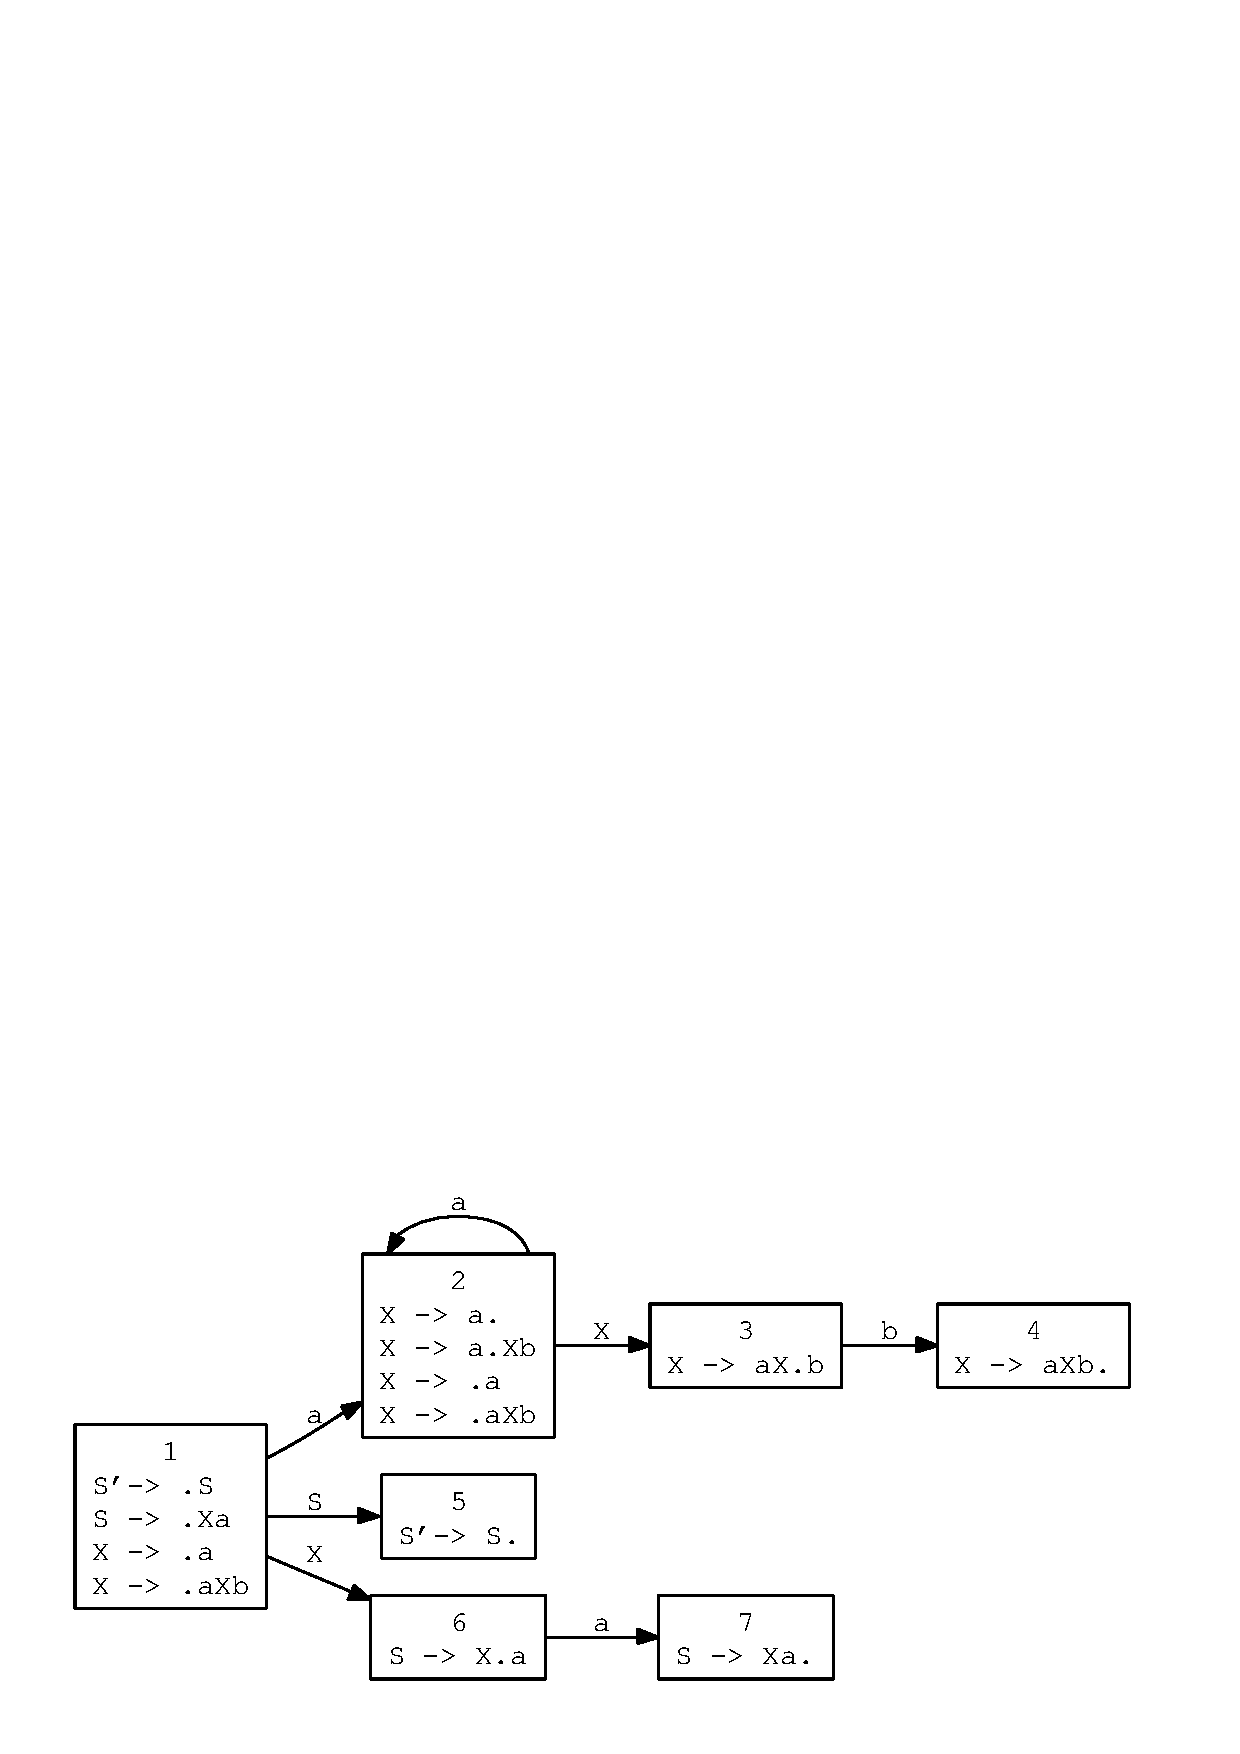
\includegraphics[scale=0.5]{viable-prefix-dfa.jpg}
				\end{center}
			\item The First and Follow sets of the non-terminals in the grammar are as follows.
				\[
					\begin{array}{ll}
						\mathrm{First}(S) = \{ \mathbf{a} \}
						& \mathrm{Follow}(S) = \{ \textbf{\$} \} \\
						\mathrm{First}(X) = \{ \textbf{a} \}
						& \mathrm{Follow}(X) = \{ \textbf{a}, \textbf{b} \}
					\end{array}
				\]
				In the DFA state $2$, one valid action for an SLR(1) parser would be
				to shift \textbf{a}.  Also, the parser could reduce using the
				production $X \rightarrow \textbf{a}$ on the lookahead symbol
				\textbf{a}, because \textbf{a} is in the Follow set of the
				non-terminal $X$.
			\item
				\[
					\begin{array}{lll}
						\mathrm{Configuration} & \mbox{DFA Halt State} & \mathrm{Action} \\
						\hline
						\mid \textbf{a a b a \$} & 1 & \mathrm{Shift} \; \textbf{a} \\
						\textbf{a} \mid \textbf{a b a \$}
						& 2 \quad \mbox{shift-reduce conflict}
						& \mathrm{Shift} \; \textbf{a} \\
						\textbf{a a} \mid \textbf{b a \$} & 2
						& \mathrm{Reduce} \; X \rightarrow \textbf{a} \\
						\textbf{a }X \mid \textbf{b a \$} & 3
						& \mathrm{Shift} \; \textbf{b} \\
						\textbf{a } X \textbf{ b} \mid \textbf{a \$} & 4
						& \mathrm{Reduce} \; X \rightarrow \textbf{a} X \textbf{b} \\
						X \mid \textbf{a \$} & 6 & \mathrm{Shift} \; \textbf{a} \\
						X \textbf{ a} \mid \textbf{\$} & 7
						& \mathrm{Reduce} \; S \rightarrow X \textbf{a} \\
						S \mid \textbf{\$} & 5 & \mathrm{Reduce} \; S' \rightarrow S \\
						S' \mid \textbf{\$} & & \mathrm{Accept}
					\end{array}
				\]
			\item The item $X \rightarrow \textbf{.}$ will appear in the DFA state 2.
				Now, in state 2, there will be two possible reductions on the
				lookahead symbol \textbf{a}: $X \rightarrow \textbf{a}$ and
				$X \rightarrow \varepsilon$.
		\end{enumerate}
	
\end{enumerate}
\end{document}
